\documentclass[tikz,border=6pt]{standalone}

\usepackage{amsmath,amssymb}
\usetikzlibrary{calc,arrows.meta}

\begin{document}
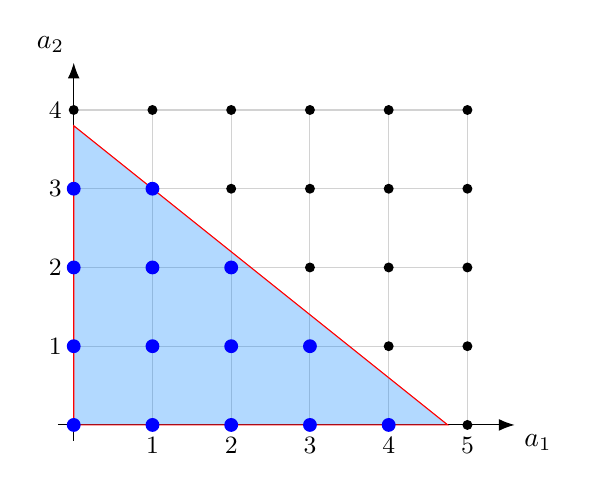
\begin{tikzpicture}[scale=1.0]
  % axes
  \draw[-{Latex[length=2mm]}] (-0.2,0) -- (5.6,0) node[below right] {$a_1$};
  \draw[-{Latex[length=2mm]}] (0,-0.2) -- (0,4.6) node[above left] {$a_2$};

  % light grid + tick labels
  \foreach \i in {1,...,5} {
    \draw[gray!35] (\i,0) -- (\i,4);
    \node[below] at (\i,-0.03) {\small \i};
  }
  \foreach \j in {1,...,4} {
    \draw[gray!35] (0,\j) -- (5,\j);
    \node[left]  at (-0.03,\j) {\small \j};
  }

  % feasible region: a1 >= 0, a2 >= 0, 4 a1 + 5 a2 <= 19
  \coordinate (O) at (0,0);
  \coordinate (B) at (0,3.8);   % 19/5
  \coordinate (C) at (4.75,0);  % 19/4
  \fill[blue!50!cyan,opacity=0.30] (O) -- (B) -- (C) -- cycle;
  \draw[red]                (O) -- (B) -- (C) -- cycle;

  % lattice points (draw AFTER fill so they sit on top)
  \foreach \i in {0,...,5} {
    \foreach \j in {0,...,4} {
      \fill[black] (\i,\j) circle (1.8pt);
    }
  }

  % feasible integer grid points: 4*i + 5*j <= 19
  \foreach \j in {0,...,3} {
    \pgfmathtruncatemacro{\imax}{floor((19 - 5*\j)/4)}
    \foreach \i in {0,...,\imax} {
      \fill[blue] (\i,\j) circle (2.5pt);
    }
  }
\end{tikzpicture}
\end{document}
